\documentclass{article}

\usepackage{ijcai13}
\usepackage{times}
\usepackage{amsmath} 
\usepackage{latexsym} 
\usepackage{ dsfont }
\usepackage{tikz}
\usepackage{circuitikz}
\usepackage{graphicx}
\usepackage{subcaption}
\usepackage{alltt}
\usepackage[ruled,vlined,linesnumbered]{algorithm2e}
\usetikzlibrary{arrows,automata, positioning, patterns}

\newtheorem{definition}{Definition}
\DeclareMathOperator*{\argmax}{arg\,max} 

\title{Bootstrap learning via modular concept discovery}

\author{Eyal Dechter \\
MIT\\
USA \\
edechter@mit.edu
\And
Jon Malmaud \\
MIT \\ 
USA \\
malmaud@mit.edu
\And 
Ryan P.  Adams \\
Harvard University\\
USA \\
rpa@seas.harvard.edu
\And
Josh Tenenbaum \\
MIT\\
USA \\
jbt@mit.edu
}

\begin{document}

\maketitle

\begin{abstract}
 Suppose a learner is faced with a domain of problems about which it
 knows nearly nothing. It does not know the distribution of problems,
 the space of solutions is not smooth, and the reward signal is
 uninformative, providing perhaps a few bits of information but not
 enough to steer it effectively. How can such a learner ever get off
 the ground? A common intuition is that if the solutions to these
 problems share a common structure, and the learner can solve some
 simple problems by brute force, it should be able to extract useful
 components from these solutions and, by composing them, explore the
 solution space more efficiently. Here, we formalize this intuition,
 where the solution space is the space of typed functional programs
 and the gained information is stored as a stochastic grammar over
 programs. We propose an iterative procedure for exploring such
 spaces: in the first step of each iteration, the learner explores a
 finite subset of the domain, guided by a stochastic grammar; in the
 second step, the learner compresses the successful solutions from the
 first step to estimate a new stochastic grammar. We test this
 procedure on symbolic regression and boolean circuit learning and
 show that the learner discovers modular concepts for these
 domains. Whereas the learner is able to solve almost none of the
 posed problems in the procedure's first iteration, it rapidly becomes
 able to solve a large number by gaining abstract knowledge of the
 structure of the solution space.
 
 
\end{abstract}

\section{Introduction}

Imagine you are trying to learn to bake via trial and error. You know
what kind of ingredients are used in baking (flour, water, butter,
sugar, yeast, baking soda, etc.) and you know a bit about how to
combine these ingredient (mix, whisk, etc.) and how to apply heat
(oven). But baking is a notoriously fragile process: ratios of
ingredients, the order of mixing, cooking temperatures, resting times,
all make a huge difference, and the outcome of the baking process is
mostly all or none. Either the outcome is what you expected or quite
unlike it. Even if you do create something similar to your intent, it
is difficult to assign blame for the outcome to any one step or
decision along the way.

Many difficult learning problems have this structure -- learning
language, developing technologies and scientific theories, learning to
play instruments or execute other complex motor patterns. These are
problems in which 1) there is a large set of similar tasks; 2) their
solutions are best described as programs; 3) the solution space is
not smooth with respect to the outcome; 4) and the outcome is generally
uninformative unless you are already pretty close to a solution.

Intuitively, the way to solve such problems is to stumble on solutions
to simple cases in the domain and extract conceptual building blocks
that can be composed to scale up to complex cases. To return to the
baking example, cookies are much simpler than cakes. There are fewer
steps to get just right. But once you have figured out a few simple
pastries, the more complex ones are mostly just variations and
combinations of techniques learned along the way. 

Of course, knowledge is not acquired wholly by trial and error. But in
many domains, there is at least initially such a period of ignorance,
and the question we are trying to tackle here is how you ever get off
the ground.

To frame this learning paradigm computationally, we make two modeling
choices. First, to emphasize the impoverished reward signals in these
domains, we model the learning task as an all-or-none optimization
problem: either the learner gets some reinforcement or she does
not. Second, to emphasize the lack of locally smooth structure in the
space of possible solutions, we choose as our solution space the space
of functional programs. These two choices are in contrast to the
paradigm tackled by most of machine learning, in which a locally
informative objective function guides search in a space that is
somewhat smooth.

%% Let a \emph{task} be a function $t : \mathcal{L} \rightarrow \{0,
%% 1\}$, where $\mathcal{L}$ is the set of all expressions in our
%% representation language. We say that $e \in \mathcal{L}$ \emph{solves}
%% task $t$ if $t(e) = 1$. Our goal is to solve as many tasks as
%% possible, as efficiently as possible. That is, suppose that there is a
%% distribution over tasks $t \sim  p_t(\cdot)$, we would like an ordering $O
%% = e_1, \dots $ on expressions in $\mathcal{L}$ such that if $p_t(t_1)
%% > p_t(t_2)$ then the first expression in $O$ to solve $t_1$ comes
%% before the first expression in $O$ to solve $t_2$.

%% We motivate a solution to this problem by considering a heirarchical
%% Bayesian formulation of the task distribution. Suppose we believe that
%% there is some underlying structure to $p_t(\cdot)$ that is explained by
%% the fact that for each task $t$ there is a latent expressions $e \in
%% \mathcal{L}$ drawn from a stochastic grammar $\mathcal{G}$ and that 

%% \begin{align}
%% e &\sim p_\mathcal{L}(\cdot) = \mathcal{G}\\
%% t | e &\sim \text{U}\{ \text{tasks solved by }e\}.
%% \end{align}

%% Then $p_t(t) = \sum_{e_j \in \mathcal{L} \text{ s.t. } t(e_j) = 1}
%% p_\mathcal{L}(e_j)$. If we make the assumption that for the set $E$ of
%% expressions in this sum, there is some expression $e^*$ such that
%% $p_\mathcal{L}(e^*) >> p_\mathcal{L}(e), e \neq e^*$, then we have, approximately, 
%% \[ p_t(t) \propto} p_\mathcal{L}(e^*). \] 

%% This suggests a way to find the ordering $O$: infer a stochastic
%% grammar $G$, under the assumption that $G$ favors one solution to a
%% given task over any other, and order the elements of $\mathcal{L}$
%% according to $G$.

%% Thus, our basic procedure will be to search for a single ``good''
%% solution for as many tasks as we can, and to use those solutions to
%% estimate a stochastic grammar. Our search will be performed in the
%% order of the most recently inferred grammar. So as our ordering
%% becomes more efficient and we can solve more tasks, we learn better
%% stochastic grammars.

%% Formally then, our goal is to solve the following minimal feedback
%% multi-task program induction problem: suppose we are given set of
%% \emph{tasks} $T=\{t_k\}_{k=1}^K$ where each task is a function $t_i :
%% \mathcal{L} \rightarrow \{0, 1\}$, where $\mathcal{L}$ is the set of
%% programs in our language.  We say that $ p \in \mathcal{L}$
%% \emph{solves} $t_i$ if $ t_i\; p = 1$. Our goal is to find a set of
%% solutions $X = \{x_k\}_{k=1}^k \subset \mathcal{L}$ such that

%% \[
%% X = \argmax_{x_1, \dots, x_K \in L} \sum_k t_k(x_k).
%% \]

Based on the motivation set out above, we present an iterative
strategy. Given a stochastic grammar $\mathcal{G}$ which defines a
distribution over the primitives from $\mathcal{L}$ and a integer
\emph{frontier size} $N$, we perform two steps in each iteration.  In
the first step, we explore the $N$ highest probability programs
according to $\mathcal{G}$. In the second step, we compress the
programs that solve any of our tasks, and we use that compression to
define a new grammar. Repeating these two steps, we effectively
reparameterize our search space to include programs that are more likely
to be solutions to our tasks. 

The remainder of this paper will include three major sections. First,
we will describe the representation language we chose and the goals of
the exploration and compressions steps. Following that, we will
discuss the algorithmic details that render our procedure
feasible. Finally, we present results from two experiments, involving
the domains of symbolic regression and boolean circuit learning.

%% \section{}
%% Let $\mathcal{F}$ be a family of distributions over $\mathcal{L}$ such
%% that for any $\mathcal{D} \in \mathcal{F}$ we can a) evaluate the
%% probability of program $p$, $P_D(p)$, and we can b) enumerate elements
%% from $D$ in descending order. 


%%  To motivate a solution to our problem, we begin with the hierarchical
%% Bayesian formulation of multi-task program induction found in Liang et
%% al.~\cite{liang10programs}. The general idea there is to estimate
%% solution programs for a set of related problems by inferring the posterior
%% distribution over solutions under the assumption that all the solution
%% programs are generated from a common latent stochastic grammar. By
%% jointly inferring solutions and the latent grammar, we find a set of
%% solutions that favors reuse of subcomponents.

%% While this framework is appealing in its elegance and Bayesian
%% interpretation, it cannot be straightforwardly adapted to the
%% situation we are considering here because their proposed MCMC
%% algorithm relies on a local log-likelihood signal, the very kind that
%% we are assuming we do not have access to.

%% To begin, we provide a high level overview of the algorithm and the
%% problem that it solves. The problem setup requires a representation
%% language for programs and a family of distributions over expressions
%% in that language, but we leave these details for the following section

\section{Extracting modular concepts from functional programs}

In order to solve our stated problem, we need to choose a solution
representation language and a compression criterion, and we need to
describe the frontier enumeration and compression procedures.

\subsection{Representing typed functional programs as binary trees}

Following~\cite{liang10programs} and~\cite{Briggs:2008}, we use
combinatory logic -- a variable-free subset of the polymorphic
simply-typed lambda calculus~\cite{Pierce_2002} -- as
our program representation language. In short, the combinatory logic
introduces a \emph{basis} of several primitive \emph{combinators} such
that any function in the lambda calculus can be alternatively written
as applications of the basis combinators. Some common basis
combinators are defined as follows:
\begin{align}
I\; x &\rightarrow  x \\
S\; f\; g\; x\; &\rightarrow (f\; x)\; (g\; x) \\ 
B\; f\; g\; x\; &\rightarrow (f\; x)\; g \\ 
C\; f\; g\; x\; &\rightarrow f\; (g\; x) \\ 
\end{align}

The basis
combinators are theoretically enough to express any Turing computable
function, but we will assume that our language has a variety of
primitives and, together with the basis combinators, we call these the
primitive combinators.

The basis combinators can themselves been expressed in the lambda
calculus. The lambda calculus has two basic operations -- application
and abstraction -- but in using the combinatory logic we sequester
uses of the abstraction operation inside the combinators, and thus
have a representation language that is effectively abstraction- and,
thus, variable-free. In doing so, we have replaced the variable
binding of the $\lambda$ operator with the variable \emph{routing} of
these basis combinators. See~\cite{liang10programs} for a more
detailed discussion of this routing interpretation. 

This is very convenient for program synthesis: since every expression
is the application of one expression to another -- with this recursion
bottoming out at the primitive combinators -- each program is a binary
tree. Most importantly, any subtree is itself a well-formed
expression; this is not the case in the lambda calculus, since
abstraction introduces long range dependencies between the $\lambda$
operator and the variables to which that operator refers. In the
lambda calculus, then, a subtree might have free variables, not bound
to any enclosing $\lambda$. 

As a simple example of our representation, consider the squaring
function $\lambda x. * x\; x $. Using two of the basis combinators
above, we can write the squaring function in combinatory logic as $S *
I$ (taking $*$ as a primitive), where application associates to the
left, so we drop the parentheses. When we apply this combinator to a
value $x$, the action of the combinator is defined as $S \;*\; I\;
x~\rightarrow~(*\; x)\; (I\; x)~\rightarrow(*\; x)\; x$.

We can extend this representation with a simple polymorphic type
system~\cite{Pierce_2002}. In this representation, a type is either a
type primitive (e.g. reals, integers, booleans, etc.), a type variable
(e.g. $\sigma$), or a function type $ t_1 \rightarrow t_2$ of
functions from source type $t_1$ to target type $t_2$. Thus, this
combinator can be represented as a binary
tree~(Figure~\ref{fig:clbintree}) whose leaves are typed primitive
combinators and whose interior nodes represent typed applications of
combinators.

\begin{figure}
  \centering
  \begin{subfigure}[Before]{0.5\linewidth}
    \begin{tikzpicture}[scale=.9,
        transform shape, level/.style={sibling distance=10mm/#1, font=\scriptsize}
        ]
      \node [font=\scriptsize] (top) {$Int$}
      child {node [above=.3cm, text width=2cm] (a) {$(Int \rightarrow Int) \rightarrow Int 
          \rightarrow Int$}
        child {node [left=.5cm, below=1cm, text width=3cm] 
          {$S : \\(t_2 \rightarrow t_1 \rightarrow t_0)  \rightarrow (t_2 \rightarrow t_1) 
            \rightarrow \\ t_2 \rightarrow t_0$}}
        child {node [right=0cm, text width=2cm] {$*: Int \rightarrow Int \rightarrow Int$}}
      }
      child {node [below right=.3cm and 1cm] (b) {$Int \rightarrow Int$}
        child {node {$I: t_0 \rightarrow t_0 \rightarrow t_0$}}
      };
    \end{tikzpicture}
    \label{fig:clbintree}
  \end{subfigure}
  \begin{subfigure}[After]{0.4\linewidth}
    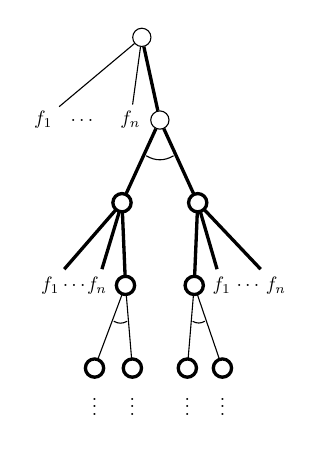
\begin{tikzpicture}[scale=.7, transform shape, 
        level/.style={sibling distance=10mm/#1},
        every edge/.style={draw, thin}
      ]
      \node [circle,draw] (a) {}
      child {node [left=0cm] (b) {$f_1$}}
      child {node [left=.2cm] (c) {\dots} edge from parent[draw=none] }
      child {node [left=.4cm] (e) {$f_n$}}
      child {node [circle,draw, left=1cm] (d) {} edge from parent[very thick]
        child {node [circle, draw, left=.25cm] (l) {} edge from parent[draw=none]
          child {node [left=.5cm] (b) {$f_1$}} 
          child {node [left=.3cm] (c) {\dots} edge from parent[draw=none] }
          child {node [left=.3cm] (e) {$f_n$} edge from parent[very thick]}
          child {node [circle, draw, left=.25cm] (and2) {}
            child {node [circle, draw, left=.25cm](l2) {} edge from parent[draw=none] 
              child {node [above=.5cm] {\vdots} edge from parent[draw=none]}
            }
            child {node [circle, draw] (r2)  {} edge from parent[draw=none] 
              child {node [above=.5cm] {\vdots} edge from parent[draw=none]}
            }
          }
        }
        child {node [circle, draw, right=.25cm] (r) {} edge from parent[draw=none]
          child {node [circle, draw, right=.25cm] (and3) {}
            child {node [circle, draw ](l3) {} edge from parent[draw=none] 
              child {node [above=.5cm] {\vdots} edge from parent[draw=none]}
            }
            child {node [circle, draw, right=.2cm ] (r3)  {} edge from parent[draw=none] 
              child {node [above=.5cm] {\vdots} edge from parent[draw=none]}
            }
          }
          child {node [right=.3cm] (b) {$f_1$} edge from parent[very thick]} 
          child {node [right=.4cm] (c) {\dots} edge from parent[draw=none] }
          child {node [right=.6cm] (e) {$f_n$}}
        }
      };
      
      \path (d)  edge[very thick]  node[inner sep=0mm,pos=.4] (a1) {} node {} (l);
      \path (d)  edge[very thick]  node[inner sep=0mm,pos=.4] (b1) {} node {} (r);
      \path (a1) edge[bend right] (b1) ;

      \path (and2)  edge node[inner sep=0mm,pos=.4] (t0) {} node {} (l2);
      \path (and2)  edge node[inner sep=0mm,pos=.4] (k0) {} node {} (r2);
      \path (t0) edge[bend right] (k0) ;

      \path (and3)  edge node[inner sep=0mm,pos=.4] (t1) {} node {} (l3);
      \path (and3)  edge node[inner sep=0mm,pos=.4] (k1) {} node {} (r3);
      \path (t1) edge[bend right] (k1) ;
    \end{tikzpicture}
    \caption{AND/OR expression search space. }
    \label{fig:andor}
    \end{subfigure}
  \caption{(a) The typed combinator $S * I$ ($f(x)=x^2$) represented as
    binary tree. (b) The space of all typed combinators represented as an
    infinitely deep AND/OR tree. Any specific combinator is a
    sub-binary tree of this AND/OR tree whose leaves consist of only
    the $f_i$ nodes (i.e., the primitive combinators of the grammar).}

\end{figure}

\subsection{A stochastic grammar over programs.}
\label{sec:stochgrammar}
A stochastic grammar over programs represents a distribution over
expressions in $\mathcal{L}$. We associate with each primitive
combinator $c_i$ in $\mathcal{L}$ a probability $p_i$,
$0~\leq~p_i~\leq~1, \sum_i~p_i~=~1 $.

We define the probability of an expression $e$ consisting of primitive
combinators $c_1, \dots, c_N$ to be $p(e)~=~\prod_{n=1}^N p(c_n |
t(c_n))$ where $t(c_n)$ is the requested type when $c_n$ was used and
\[
p(c_i | t(c_n)) =    \frac{1}{4}\frac{p_i}{\sum_{c_j :
    type(c_j) \text{ unifies with } t(c_n)} p_j}.
\]
That is, $p(c_i | t(c_n)$ is the probability of sampling $c_i$ from
the multinomial distribution defined by the $p_i$'s, conditioned on
the requesting type, and then divided by 4. The constant factor of
$1/4$ is introduced as a simple way to ensure that the sum over the
probabilities of all expressions converges to finite value (so that
the distribution over expressions is proper).\footnote{The probability
  mass $M_d$ of all expressions of depth less than or equal to $d$ can
  be written with the recurrence relation $M_d \leq M_d^2 + M_1$. This
  has an asymptotic fixed point if $x = x^2 + M_1$ has a solution,
  which is true if $M_1 \leq 1/4$.}

To estimate the values $p_i$ from set of expressions, we simply divide
the number of times primitive combinator $c_i$ was used by the number
of times it could have been used given the requesting types in the
expression trees. Note that this is not a maximum likelihood estimator
for this distribution; finding that would require solving a rather
complex optimization problem because of each choice is conditioned on
the requesting type. We choose our estimator merely for convenience,
and find that our empirical results justify this simplicity. It is a
matter for future research to determine to what extent a more accurate
estimator would improve performance.

 \subsection{Best-first enumeration of most probable programs.}
In order to explore the frontier of most promising programs, we need a
procedure that enumerates the $N$ most probable programs. There has
been recent interest in this problem, most of it focused on
enumerating the shortest program satisfying some
criterion~\cite{DBLP:conf/sfp/Katayama05} \cite{DBLP:conf/aaip/YakushevJ09}. Our
approach is to formulate the problem as a best-first exploration of an
AND/OR tree~\cite{nilsson1982principles}, which we denote
$\mathcal{G}$. A complete program is any binary subtrees of
$\mathcal{G}$ whose leaves coincide with the leaves of
$\mathcal{G}$. The tree structure is shown in
Figure~\ref{fig:andor}. The root is an OR node of the requisite
program type. It's children are the primitives of that type $f_1,
\dots, f_n$, and one AND node with two children. Each child of an AND
node has the same structure as the root node, with modified types: if
the type of an AND node is $t$, then the type of its left child is
$\tau \rightarrow t$ (where $\tau$ is a fresh type variable). Since
the type of the right child is constrained by the subtree rooted at
the left child, we always expand the left child first and use the
target type of this left subtree to mark the type of the right child.

Recall that a valid partial solution is a subtree of $\mathcal{G}$
satisfying the following properties: its root is the root
$\mathcal{G}$ and any OR node has at most one child. A complete
solution is a partial solution whose leaves are leaves of
$\mathcal{G}$, whose root is the root of $\mathcal{G}$, in which each
OR node has exactly one child, and in which each AND node has exactly
two children. 

The value of a partial solution $G'$ is calculated by summing the
value of its leaves. If a leaf of $G'$ is a leaf of $G$ then either it
is an AND node, to which we assign a value of 0, or it corresponds to
some primitive combinator $c_i$ in the library and is the child of
some typed OR node with type $t$. We assign its value of $- \log{p(c_i
  | t)}$, according to the stochastic grammar specified in
Section~\ref{sec:stochgrammar}. If a leaf $v$ of $G'$ is an OR node,
then the value of any extension of it to a complete solution is at
most $-log(1/4)$. Thus, we have defined a value for partial solutions
that upper bounds the value of any of its extensions. 

Our best-first policy, is to simply expand the next partial solution
with the highest value. If a partial solution has multiple leaves that
are not primitive combinators, we expand the left most one first,
since it is the choice of left combinator that defines the type of its
right combinator in an application pair. That is, the parent node
applies its constraint on valid solutions via the left child, not the
right child. We want to apply constraints as early as possible, so
expanding left children first prunes more partial solutions.

\textbf{****NEED COMPLEXITY ANALYSIS HERE*******}

\subsection{Finding the most compressive set of solutions.}

We say that a task is \emph{hit} if it has a solution in the
frontier. Having enumerated the frontier, we want to assign solutions
to hit tasks such that this set is maximally compressible. This will
promote the usage of reusable modular subtrees. 

A natural metric for the compressibility of a set of binary trees is
the number of unique subtrees that this set contains. As an example of
this, suppose we had three tasks whose solutions were integers 16, 25,
and 36, and suppose our frontier contained the six expressions:

%% \begin{figure}[h]
%%     \begin{tikzpicture}[scale=.9,
%%         transform shape, level/.style={sibling distance=10mm/#1, font=\scriptsize}
%%         ]
%%       \node [font=\scriptsize] (top) {}
%%       child {node [above=.3cm, text width=2cm] (a) {$(Int \rightarrow Int) \rightarrow Int 
%%           \rightarrow Int$}
%%         child {node [left=.5cm, below=1cm, text width=3cm] 
%%           {$S : \\(t_2 \rightarrow t_1 \rightarrow t_0)  \rightarrow (t_2 \rightarrow t_1) 
%%             \rightarrow \\ t_2 \rightarrow t_0$}}
%%         child {node [right=0cm, text width=2cm] {$*: Int \rightarrow Int \rightarrow Int$}}
%%       }
%%       child {node [below right=.3cm and 1cm] (b) {$Int \rightarrow Int$}
%%         child {node {$I: t_0 \rightarrow t_0 \rightarrow t_0$}}
%%       };
%%     \end{tikzpicture}
%% \end{figure}

Let $|e|$ be the
number of unique binary trees in expression $e$. 

we will find that some tasks have no solutions
and some have one or more solutions; for those tasks that have
solutions, we want to choose a solution for each task such that the
complete set of such solutions for all solved tasks is as compressible
as possible.


Thus, we can attempt
to find the assignment of solutions to tasks that minimizes this
value. However, an exact optimization for this problem requires
examining $O(m^k)$ assignments, where $m$ is the maximum number of
solutions for any one task and $k$ is the number of tasks. Since this
is prohibitive, we relax the compressibility metric as follows: we
define the cost of adding each new solution $s_n$ to a partial set of
solutions $s_1, \dots, s_{n-1}$ to be the number of additional unique
subtrees in $s_n$ that are not present in $s_{n-1}$. Our solution thus
becomes approximate and that approximation is order-dependent, but a
depth-first search on the defined search space goes from exponential
in the solution degree to quadratic.

\subsection{Re-estimating the stochastic grammar over programs.}

Given a set of solution programs, we want to re-estimate our
stochastic grammar. Our inspiration for doing this is based broadly on
the Neville-Manning algorithm for grammar-based
compression~\cite{nevill1997identifying}. The idea of that compression
algorithm is to compress any string by creating a grammar for that
string such that a) no two symbols appear more than once in the
grammar and b) every rule is used more than once. From a set of trees
we generate a grammar according to these criteria (though using a less
efficient and much simpler algorithm). 

In our algorithm, we traverse a set of combinator binary trees in
depth first order. We count the occurrences of every subtree. Every
time we encounter a subtree for the \emph{second} time, we designate
it as a primitive in our new grammar. This ensures that every
primitive is used more than once. During our traversal, we do not
descend into trees that have been added already to the new
grammar. Thus, we only count an instance of tree if that instance is
not a subtree of a primitive element of the new grammar.

At the end of this traversal of the solution programs, we have a parse
of the solution set with a new set of primitives and we know how many
times each primitive occurred in the solutions set. To estimate the
probabilities associated with each node production, we again traverse
the solution set, but this time for each node we count which other
primitive elements from the new grammar could have been used. We
estimate the terminal production weight to be the ratio of the number
of times that node was used in the first traversal divided by the
number of times it was used in the second traversal. 

Note that this probability estimation procedure was chosen for its
simplicity, and it is not the maximum likelihood estimator for the
multinomial distribution according to which we enumerate the
data. Because the probability we assign to the use of a primitive
combinator depends on the type of the node, the ML estimator of the
probability of that combinator is not a simple ratio of counts. It
would be interesting to determine whether a more accurate estimator
can improve this algorithm's performance.

\section{Experiments.}
\subsection{Symbolic regression.}
\label{sec:symreg}

In this section, we walk through the performance of our learning
algorithm on a symbolic regression problem. In this problem,
each task is a set of pairs $ (x, f(x))$ where $x \in (0, \dots, 10)$
and $f$ is a polynomial. The goal is to discover a program for each
task that outputs the appropriate value $f(x)$ for each input x. We
assume that the data is noise-free.


%% The choice of an initial grammar for the algorithm will, of course,
%% have a big effect on its performance, and so we would like to
%% characterize this effect. We can divide primitives into roughly two
%% sets; there are low-level primitives, those that operate on concrete
%% types like Bool or Double, and these tend to be domain specific. For
%% example, concrete primitives include $1, 2$, etc., and $f(x) = 3x$. The
%% other class of primitives are abstract primitives, which can be
%% characterized by having arguments whose types are primarily function
%% types, like $(t \rightarrow s), (t \rightarrow s) \rightarrow \text{
%%   Double },$ etc. Of course, we can construct operators that fall in
%% between. 

%% The most abstract operators are those that Liang et. al refer to as
%% ``routers''~\cite{liang10programs}. These operators take the place of
%% $\lambda$ abstraction in the general lambda calculus: whereas
%% $\lambda$ abstraction allows us to bind arguments to variables nested
%% deep inside an expression, without them we need to have operators that
%% ``route'' arguments to the appropriate functions in a nested
%% expression. 

%% \begin{definition}[Router~\cite{liang10programs}] A \emph{router} is a combinator
%% represented by a finite sequence of elements from $\{B, C, S\}$. The
%% behavior of router $r$ is given by
%% \[
%% (r \, f \, g \, x_1 \dots x_{|r|}) = (f \, x_{i_1} \dots x_{i_n}) (g
%% \, x_{j_1} \dots x_{j_n}),
%% \]
%% where $i_1 < \dots < i_n$ are indices $i$ such that $r_i \in \{C, S\}$
%% and where $j_1 < \dots < j_n$ are indices $j$ such that $r_j \in \{B,
%% S\}$. Let $\mathcal{R}_k$ be the set of all routers of length equal to
%% $k$. Let $\mathcal{R}_{\leq k}$ be the set of all routers of length
%% less than or equal to $k$.
%% \end{definition}

%% To analyze the behavior of our algorithm, we will vary the parameters
%% of the problem along two axes while keeping the learning tasks the
%% same. Along the first axis, we vary the initial library to which our
%% learner has access with respect to the its abstractness (i.e., number
%% of routers) and its concreteness (i.e. number of concrete
%% primitives). Along the second axis we vary the size of the search
%% frontier.

Each task is to predict the value of an unknown polynomial on the
inputs $0, \dots, 10$. The set of tasks corresponds to the set of
polynomials $\{ax^2 + bx + c | a, b, c \in \{0, \dots, 10 \}\}$. The
choice of primitives is going to make a big difference in performance;
we chose to include the basic combinators I, S, B, C and four
arithmetic primitives, $1$, $0$, $*$, and $+$. The choice of initial
weights makes a large difference as well, as it determines the
relative ordering of combinators in the enumeration step. To get a
general sense of the algorithm's performance, we set the intial
weights to be slightly different on each run, jittering them around a
uniform weighting.

In Figure~\ref{fig:symreg}, we show performance results as we vary the
frontier size. Each individual plot shows how changing the frontier
size changes the number of tasks the algorithm identifies correctly
over the course of fifteen algorithm iterations. %% In addition, we have a
%% baseline for each curve, visits the same number of expressions as the
%% corresponding algorithm run (i.e. frontier size $\times$ $\#$ of
%% iterations) but all at once; it does not do any learning. Thus, this
%% baseline serves as a brute-force control for the learning aspect of
%% the algorithm.

\begin{figure}
\begin{subfigure}[Before]{.6\linewidth}
%% 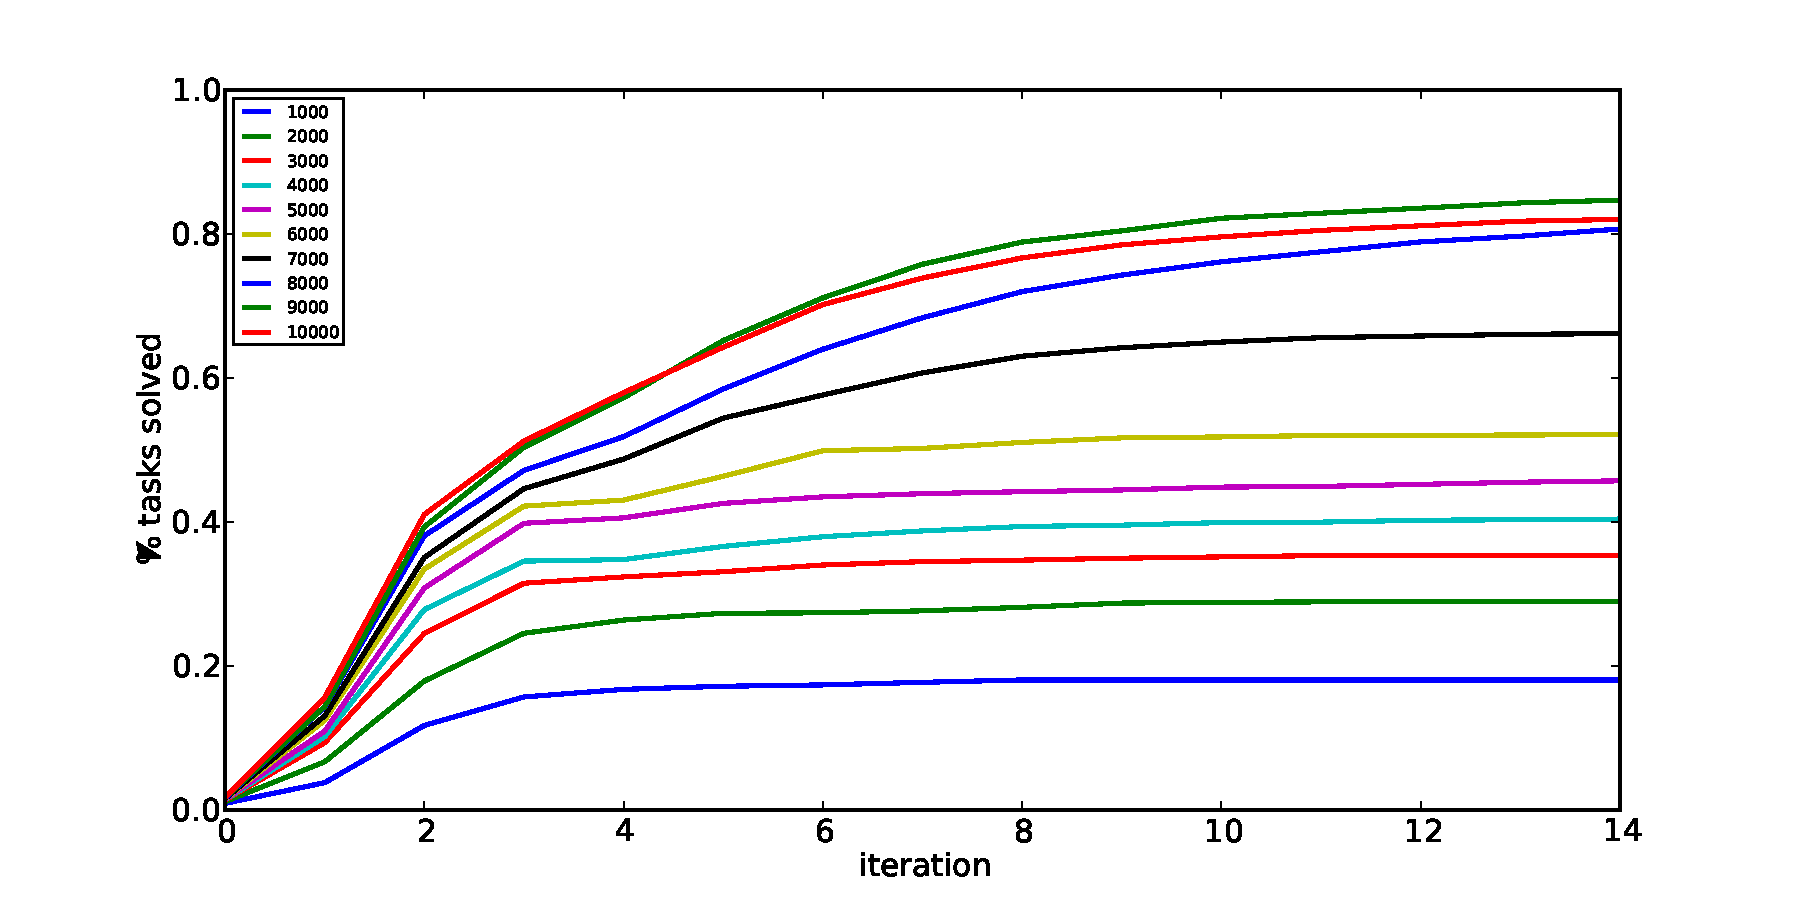
\includegraphics[width=\linewidth]{figures/learningCurves2.pdf}
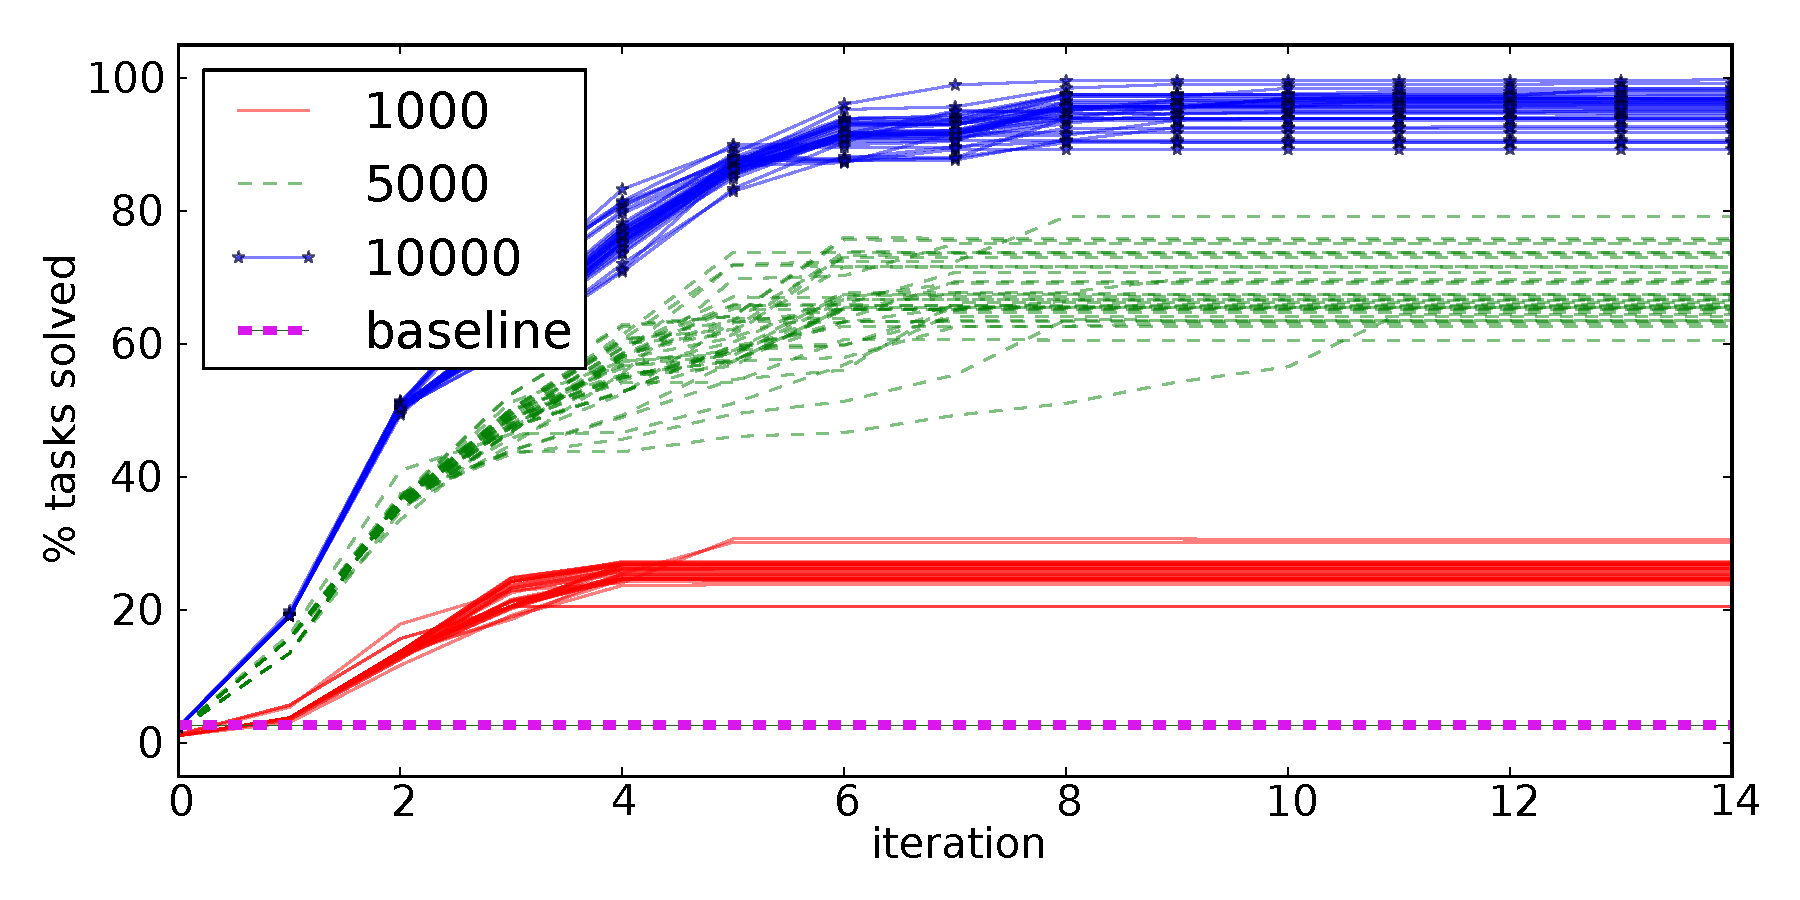
\includegraphics[width=\linewidth]{figures/symreg3frontiers.pdf}
\end{subfigure}
%% \begin{subfigure}[After]{0.45\linewidth}
%% \includegraphics[width=\linewidth]{figures/performanceVsFrontierSize2.pdf}
%% \end{subfigure}
\caption{(a) Average learning curves as we vary the frontier size. (b)
  Percent of tasks solved at iteration 15 as a function of frontier
  size.}
\label{fig:symreg} 
\end{figure}

%% Why do the learning curves asymptote early? One might object that a
%% learning algorithm should continuously improve, if only slowly, as it
%% is given more time. But in these runs we observe a finite and
%% permanent performance cap. This is expected: once the learner find a
%% set of concepts it can explain, if those concepts fill up the
%% frontier, then there is nothing to spur the learner to incorporate as
%% yet unsolved tasks. 

%% To investigate whether this is in fact the case, we can examine the
%% proportion of expressions in the frontier that match tasks in our task
%% set; that is, is the learning curve plateauing because the frontier is
%% heavily redundant, or is it plateuing because the frontier contains
%% many expressions that do not hit the task set at
%% all? Figure~\ref{fig:plateau_investigation} shows the proportion of
%% the expressions in the frontier that hit a task as the frontier size increases.

\subsection{Boolean circuits}
\label{sec:boolcircuits}

As another demonstration of this approach, we investigate the
procedure's ability to learn boolean functions using only the logical
primitive NAND and the basic combinators. It is well known that a
boolean circuit can be constructed for any boolean function given only
the NAND gate. Here, the basic combinators take the place of the
wiring normally found in a circuit, the output of element to multiple
inputs downstream. 

We constructed two task sets. The first of these was constructed
explicitly to contain familiar module structure. In this set of tasks,
we sampled $1000$ boolean circuits using AND, OR, and NOT gates. To
accomplish this, we first sampled either 1, 2, 3 inputs, then between
1 and 5 gates, randomly wiring the inputs of each new gate to the
output of one of the existing gates in the circuit. We continued this
sampling procedure until we had 1000 ``connected'' circuits, i.e.,
circuits all of whose output are wired to an input except for the last
one (the output gate). This resulted in $1000$ tasks consisting of
$82$ unique boolean functions, with a distribution of tasks as shown
in Figure~\ref{fig:booldistr}. In Figure~\ref{fig:boolLearningCurves1},
We present learning curves for frontier sizes 100, 500 and 10000,
using the same procedure as in Section~\ref{sec:symreg}. 

\begin{figure}
\includegraphics[width=\linewidth]{figures/circuitDistrComp.pdf}
\label{fig:booldistr}
\caption{Distribution of boolean functions among (a) the set of 1000
  circuits randomly constructed from AND, OR and NOT gates; b) the
  first 1000 expressions from the grammar over programs \emph{before}
  learning; c) the first 1000 expressions from the grammar over
  programs \emph{after} learning.}
\end{figure}

This problem is particularly suitable for inspecting the constituents
of the induced grammar $\mathcal{G}$. We might hope that our algorithm
recovers the consituent logic gates that were used to build up the
problems. Table~\ref{table:bool} shows a few of the top ranked
expressions in the library. These include the basic logic gates; we
also include one higher-order expression $F$, to stress that the
representation we are using allows one to build concepts that are more
expressive that just sub-circuits.

In a second experiment, we include all $272$ boolean truth tables with
three or fewer inputs as tasks. This is a more difficult problem. Note
that in the first boolean function problem, there are two kinds of
learning that can take place: first, many expressions map to a single
boolean function, so we need to learn primitives that allow us to span
many different functions instead of allows generating very simple
functions over and over again. The second kind of learning involves
the distribution of the functions themselves. In the first boolean
experiment, that structure is apparent in the distribution in
Figure~\ref{fig:boolhist}. In this second experiment, we remove the
second kind of structure. In Figure~\ref{boolLearningCurves}, we show
10 runs of the algorithm with a frontier size of $2000$: note how
there are several local minima that majority of the runs get stuck in
with performance around $50\%$, but several of the runs seem to take
different trajectories to more successful representations. 

\begin{figure}
\begin{subfigure}[Before]{0.45\linewidth}
\includegraphics[width=.9\linewidth]{figures/booleancircuitsBars.pdf}
\end{subfigure}
\begin{subfigure}[Before]{0.45\linewidth}
\includegraphics[width=.9\linewidth]{figures/boolLearningCurves.pdf}
\end{subfigure}
\caption{(a) Average learning curves as we vary the frontier size. (b)
  Percent of tasks solved at iteration 15 as a function of frontier
  size.}
\label{fig:boolLearningCurves} 


\end{figure}

\begin{table}
\scriptsize
  \begin{tabular}{|l|l|l|}
    function  & CL expressions & circuit  ~ \\ \hline
        TRUE  & (S NAND) (S NAND I)                   & ~ \\ \hline
        FALSE & (S B (S NAND)) (S NAND I)             & ~ \\ \hline
        NOT   & S NAND I                              & \begin{circuitikz}[scale=1, transform shape] \draw
(0, 0) node[left=.25] (x) {x}
(x) node[right=1cm, nand port, thick, scale=.5] (nand) {}
(nand) node[right=1cm] (out) {}
(x) -| (nand.in 1)
(x) -| (nand.in 2)
(nand) -- (out);
\end{circuitikz}
 \\ \hline
        AND   & ((C B NAND) (B (S NAND I)))           & ~ \\ 
        OR    & ((B (C (B (S NAND) NAND))) (S NAND I) & ~ \\ 
        XOR   & ~                                     & ~ \\ 
        F     & S B (S NAND)                          & \begin{circuitikz} \draw
(1, 0) node[left=.25] (x) {x}
(x) node[right=.4cm, text_align=center, draw, text width=.5cm, 
    text height=.25cm, align=center] (f1) {f}
node[below right=0.25cm and 1.0cm of f1, nand port, thick, scale=.5] (nand) {}
(nand) node[right=.4cm, text_align=center, draw, text width=.5cm, 
  text height=.25cm, align=center] (f2) {f}
(f2) node[right=.4cm] (out) {}

(x) -- (f1)
(f1) -| (nand.in 1)
(x) -| (1, -.63) -- (nand.in 2)
(nand) -- (f2)
(f2) -- (out);
\end{circuitikz}

    \end{tabular}
\caption{Expressions in the induced library on sets of tasks
  corresponding to boolean circuits synthesized from AND, OR, and NOT
  gates, with boolean circuits of 1, 2, or 3 inputs.}
\label{table:boolexpr}
\end{table}

%% \subsection{Digital arithmetic}
%% Having demonstrated the behavior of the E-C algorithm on symbolic
%% regression, we analyze its performance on tasks involving digital
%% arithmetic, a class of problems with known modular structure. The
%% general goal is to discover boolean circuits consisting of a limited
%% set of gates that perform arithmetic operations on binary number
%% representations. 

\subsection{Discussion}
This work attempts to bring together ideas from various areas of
research -- hierarchical Bayes, learning to learn, minimum description
length learning -- to provide a proof of concept that learning
abstractions from programs via compression can rapidly improve search
performance. We emphasize this by focusing on domains in which the
solution space is not smooth and the error signal is all or
none. Thus, the main source of information for learning is the modular
and compositional structure of the solution space.

Of course, the representations that people use to learn in the world
often have a partially smooth or local structure. Techniques in AI and
machine learning commonly use smoothness or local structure to make
search tractable. But the difference between this kind of learning and
conceptual learning is undeniable. The former is what the statistician
or machine learning researcher implements. The latter is what she
learns as a student and as a practicioner. As researchers, we try
different models, watch them fail or succeed, and abstract out the
elements of these models that capture the relevant differences. We mix
and match parts of different ideas, and utilize succcessful patterns
of reasoning that can span many problems and domains. 

We believe that the primary characteristic of conceptual learning is
that it occurs over a modular and compositional computational
representation that supports higher-order functions. That is why we
chose a functional programming language as the representational
language of this work.

The experiments in this work do not contain the richness of real world
learning, but we believe that the learning algorithm's behavior
exhibits some of the characteristics we would expect of a conceptual
learner. 

One characteristic of this algorithm's behavior is a rapid initial
increase in performance followed by a hard plateau. This plateau is
expected given the circular nature of the algorithm: the learner
inspects the region of the solution space that is typical of solutions
already found. We see in this phenomenon a conceptual demarcation of
the problem space: a coherent set of concepts or problems solving
techniques can define by their power the extent of problems a problem
solver is willing to consider. One might hope, however, that an
intelligent learner would recognize that such a demarcation has
occured and attempt to find another class of concepts for the
remaining unsolved tasks.

Another aspect of conceptual learning that we see present in this
algorithm's behavior is the importance of a curriculum. By this we do
not mean an explicit ordering of the problems in the task set, but
rather that a set of sufficiently simple problems must act as stepping
stones to the acquisition of complex representations. 




%% The file named.bst is a bibliography style file for BibTeX 0.99c
\bibliographystyle{plain}
\bibliography{ijcai13}
\nocite{*}

\end{document}

